\documentclass{beamer}
\usepackage{listings}
\usepackage[utf8]{inputenc} % special characters, my name, etc.
\usepackage{pslatex}	% postscript fonts
\usepackage{color}
\usetheme[nat,colourful]{Frederiksberg}

\lstset{language=C,
                basicstyle=\ttfamily,
                keywordstyle=\color{blue}\ttfamily,
                stringstyle=\color{red}\ttfamily,
                commentstyle=\color{green}\ttfamily,
                morecomment=[l][\color{magenta}]{\#}
}

\lstdefinestyle{customc}{
  belowcaptionskip=1\baselineskip,
  breaklines=true,
  frame=L,
  xleftmargin=\parindent,
  language=C,
  showstringspaces=false,
  basicstyle=\footnotesize\ttfamily,
  keywordstyle=\bfseries\color{green!40!black},
  commentstyle=\itshape\color{purple!40!black},
  identifierstyle=\color{blue},
  stringstyle=\color{orange},
}
\lstset{escapechar=@,style=customc}

\definecolor{codegreen}{rgb}{0,0.6,0}
\definecolor{codegray}{rgb}{0.5,0.5,0.5}
\definecolor{codepurple}{rgb}{0.58,0,0.82}
\definecolor{backcolour}{rgb}{0.95,0.95,0.92}

\lstdefinestyle{mystyle}{
    backgroundcolor=\color{backcolour},
    commentstyle=\color{codegreen},
    keywordstyle=\color{magenta},
    numberstyle=\tiny\color{codegray},
    stringstyle=\color{codepurple},
    basicstyle=\footnotesize,
    breakatwhitespace=false,
    breaklines=true,
    captionpos=b,
    keepspaces=true,
    numbers=left,
    numbersep=5pt,
    showspaces=false,
    showstringspaces=false,
    showtabs=false,
    tabsize=2
}

\lstset{style=mystyle}



\title{The study of MIPS32 processor simulation}
\subtitle{Presentation}
\author{Jan Mezník\\pzj895@alumni.ku.dk}
\institute{Copenhagen University}
\date{\today}




\begin{document}

% Frontpage
\frame[plain]{\titlepage}

% Table of contents
\begin{frame}
\frametitle{Outline}
\tableofcontents
\end{frame}


\begin{frame}
	\frametitle{Problem statement}
	\textit{Is it possible to implement a simulator, to fully support the
		current version of KUDOS?}\\
\end{frame}

\begin{frame}
	\frametitle{Learning objectives}

	\begin{itemize}
		\item Gain deeper understanding of the MIPS32 architecture, and
		the choices thereof

		\item How the CPU communicates and interacts with its IO devices

		\item Discover how operating systems, such as KUDOS, interacts
		with the CPU

		\item Learn the advantages and disadvantages of the MIPS architecture
		compared to other architectures, such as x86.
	\end{itemize}
\end{frame}

\begin{frame}
	\frametitle{Problem Analysis}
	KUDOS is based on the BUENOS operating system, originally developped at
	Aalto University, Finland.

\begin{block}{Requirements}
	\begin{itemize}
		\item Translation Lookaside Buffer
		\item Memory Management Unit
		\item I/O devices
		\item Pipeline
	\end{itemize}
\end{block}
\begin{block}{Optional}
	\begin{itemize}
		\item SMP (multicore)
		\item Caches
	\end{itemize}
\end{block}
\end{frame}



\begin{frame}
	\frametitle{Implementation}
	\begin{center}
	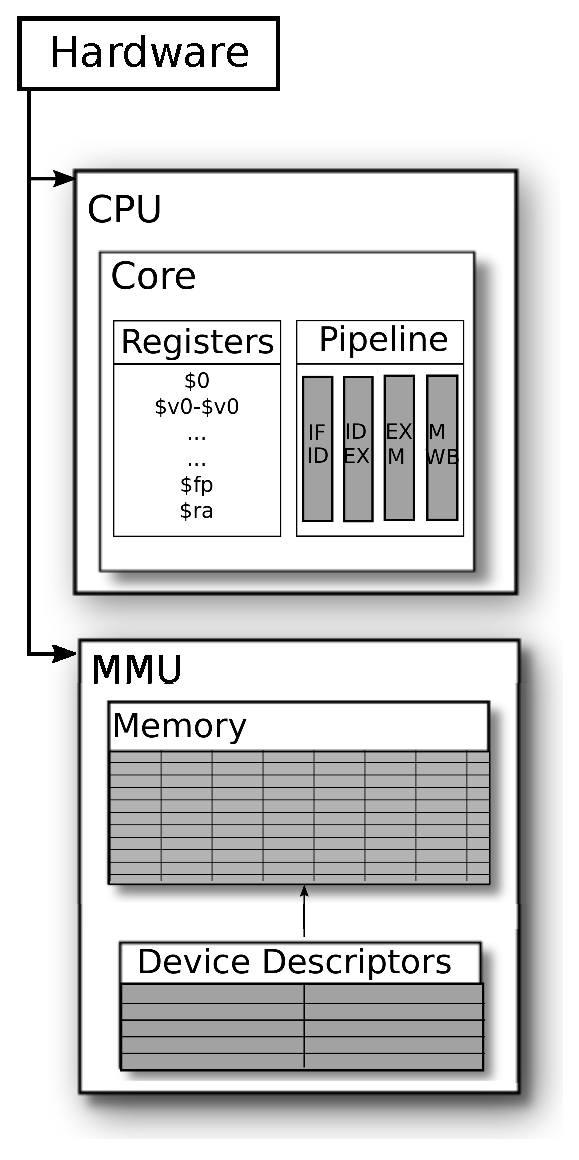
\includegraphics[scale=0.35]{../pipeline/structure_layout.eps}
	\end{center}
\end{frame}

\begin{frame}[fragile]
\frametitle{Pipeline}
\begin{columns}
\begin{column}{0.5\textwidth}

\begin{itemize}
	\item<1> Pipeline registers
	\item<2> Other stuff
\end{itemize}

\end{column}

\begin{column}{0.5\textwidth}

\begin{lstlisting}<1>
typedef struct reg_ex_mem {
	bool c_reg_write;
	bool c_branch;
	bool c_mem_read;
	bool c_mem_write;
	bool c_mem_to_reg;


	uint32_t eff_addr;
	uint32_t alu_res;

	uint32_t rt_value;
	uint8_t reg_dst;
	uint32_t next_pc;

	uint32_t inst;

	exception_t exception;
} ex_mem_t;


\end{lstlisting}


\end{column}
\end{columns}

\end{frame}


\begin{frame}
\frametitle{Results}



\end{frame}


\begin{frame}
\frametitle{Conclusion}
\end{frame}


\end{document}
